%%%%%%%%%%%%%%%%%%%%%%%%%%%%%%%%%%%%%%%%%%%%%%%%%%%%%%%%%%%%%%%%%%%%%%
% LaTeX Example: Project Report
%
% Source: http://www.howtotex.com
%
% Feel free to distribute this example, but please keep the referral
% to howtotex.com
% Date: March 2011 
% 
%%%%%%%%%%%%%%%%%%%%%%%%%%%%%%%%%%%%%%%%%%%%%%%%%%%%%%%%%%%%%%%%%%%%%%
% How to use writeLaTeX: 
%
% You edit the source code here on the left, and the preview on the
% right shows you the result within a few seconds.
%
% Bookmark this page and share the URL with your co-authors. They can
% edit at the same time!
%
% You can upload figures, bibliographies, custom classes and
% styles using the files menu.
%
% If you're new to LaTeX, the wikibook is a great place to start:
% http://en.wikibooks.org/wiki/LaTeX
%
%%%%%%%%%%%%%%%%%%%%%%%%%%%%%%%%%%%%%%%%%%%%%%%%%%%%%%%%%%%%%%%%%%%%%%
% Edit the title below to update the display in My Documents
%\title{Project Report}
%
%%% Preamble
\documentclass[paper=a4, fontsize=11pt]{scrartcl}
\usepackage[T1]{fontenc}
\usepackage{fourier}

\usepackage[protrusion=true,expansion=true]{microtype}	
\usepackage{amsmath,amsfonts,amsthm} % Math packages
\usepackage[pdftex]{graphicx}	
\usepackage{url}
\usepackage[brazil]{babel}
\usepackage[utf8]{inputenc}
\usepackage[T1]{fontenc}


%%% Custom sectioning
\usepackage{sectsty}
\allsectionsfont{\centering \normalfont\scshape}


%%% Custom headers/footers (fancyhdr package)
\usepackage{fancyhdr}
\pagestyle{fancyplain}
\fancyhead{}											% No page header
\fancyfoot[L]{}											% Empty 
\fancyfoot[C]{}											% Empty
\fancyfoot[R]{\thepage}									% Pagenumbering
\renewcommand{\headrulewidth}{0pt}			% Remove header underlines
\renewcommand{\footrulewidth}{0pt}				% Remove footer underlines
\setlength{\headheight}{13.6pt}


%%% Equation and float numbering
\numberwithin{equation}{section}		% Equationnumbering: section.eq#
\numberwithin{figure}{section}			% Figurenumbering: section.fig#
\numberwithin{table}{section}				% Tablenumbering: section.tab#


%%% Maketitle metadata
\newcommand{\horrule}[1]{\rule{\linewidth}{#1}} 	% Horizontal rule

\title{
		%\vspace{-1in} 	
		\usefont{OT1}{bch}{b}{n}
		\normalfont \normalsize \textsc{Universidade Federal do Ceará} \\ [25pt]
		\horrule{0.5pt} \\[0.4cm]
		\huge Reconhecimento de Padrões \\
		\horrule{2pt} \\[0.5cm]
}
\author{
		\normalfont 								\normalsize
        João Rafael Barbosa de Araujo\\[-3pt]		\normalsize
        \today
}
\date{}


%%% Begin document
\begin{document}
\maketitle

Esse relatório contém um curto resumo das diferentes técnicas de validação e classificação utilizados no trabalho, assim como os resultados das diferentes técnicas aplicadas ao banco de dados \textit{iris\_log}.

\section{\textit{Cross-validation}}

Validação cruzada é uma de várias técnicas que é utilizada para estimar a qualidade de generalização de um algoritmo a partir da separação de um conjunto de dados. Seu principal objetivo é quantificar a eficiência de um modelo para a chegada de novos dados além de permitir a detecção de problemas como \textit{overfitting} (uma especialização excessiva no conjunto de dados perdendo assim a capacidade de generalização do modelo) . Em um modelo preditivo é típico haver dois grupos de dados: Dados de treinamento, dados de teste. Há diversas técnicas comumente utilizadas para realizar a validação cruzada

Validação cruzada é composta pela decomposição de um conjunto de dados em subconjuntos de treinamento e teste, podendo também incluir subconjunto de validação. O primeiro subconjunto, de treinamento, será o grupo utilizado para alimentar o modelo. Já o subconjunto, de teste, será utilizado para avaliar a porcentagem de acerto do modelo comparado a classificação do modelo com a classificação real. O ultimo conjunto, de validação, é utilizado em alguns classificadores como referencia para detectar \textit{overfitting} como por exemplo em redes neurais. Uma regra de ouro da validação cruzada diz que os conjuntos de treinamento, teste e validação não devem possuir elementos em comum! As sub-sessões abaixo exemplificam os métodos de validação cruzada utilizadas no trabalho de Reconhecimento de padrões.

\subsection{\textit{Leave-one-out}}
Esse método de é um dos mais simples de ser implementado. Ele consistem em utilizar o conjunto completo menos uma amostra para o subconjunto de treinamento, e apenas essa amostra que não foi incluída no grupo de treinamento para ser o subconjunto teste. Para um conjunto de N pontos, são utilizados N subconjuntos de treinamento/teste, e a eficiência do modelo é dada em porcentagem pela média de acertos. como é mostrado na Figura \ref{fig:loo}.

\begin{figure}[h]
    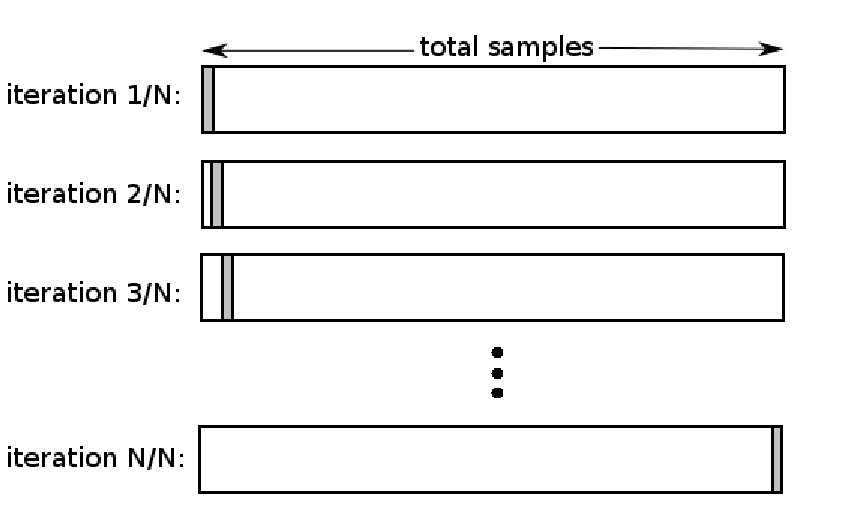
\includegraphics[width=8cm]{img/Leave-One-Out-Cross-Validation.png}
    \centering
    \caption{Validação cruzada \textit{leave-one-out}}
    \label{fig:loo}
\end{figure}

\subsection{\textit{k-fold}}

O \textit{k-fold} pode ser visto como uma extensão do \textit{leave-one-out} porém ao invés de utilizar uma única amostra para o conjunto de teste, os dados serão divididos em K conjuntos de aproximadamente mesmo tamanho. Similarmente ao que foi mostrado na sub-sessão anterior, esse método é utilizado para estimar o quão eficaz o modelo será ao encontrar dados novos, ou seja, quantificar a eficiência de uma técnica de classificação. A figura \ref{fig:kfold} mostra a divisão dos dados, onde cada bloco (\textit{train/test}) contem \textbf{k} conjuntos de aproximadamente mesmo tamanho.

\begin{figure}[h!]
    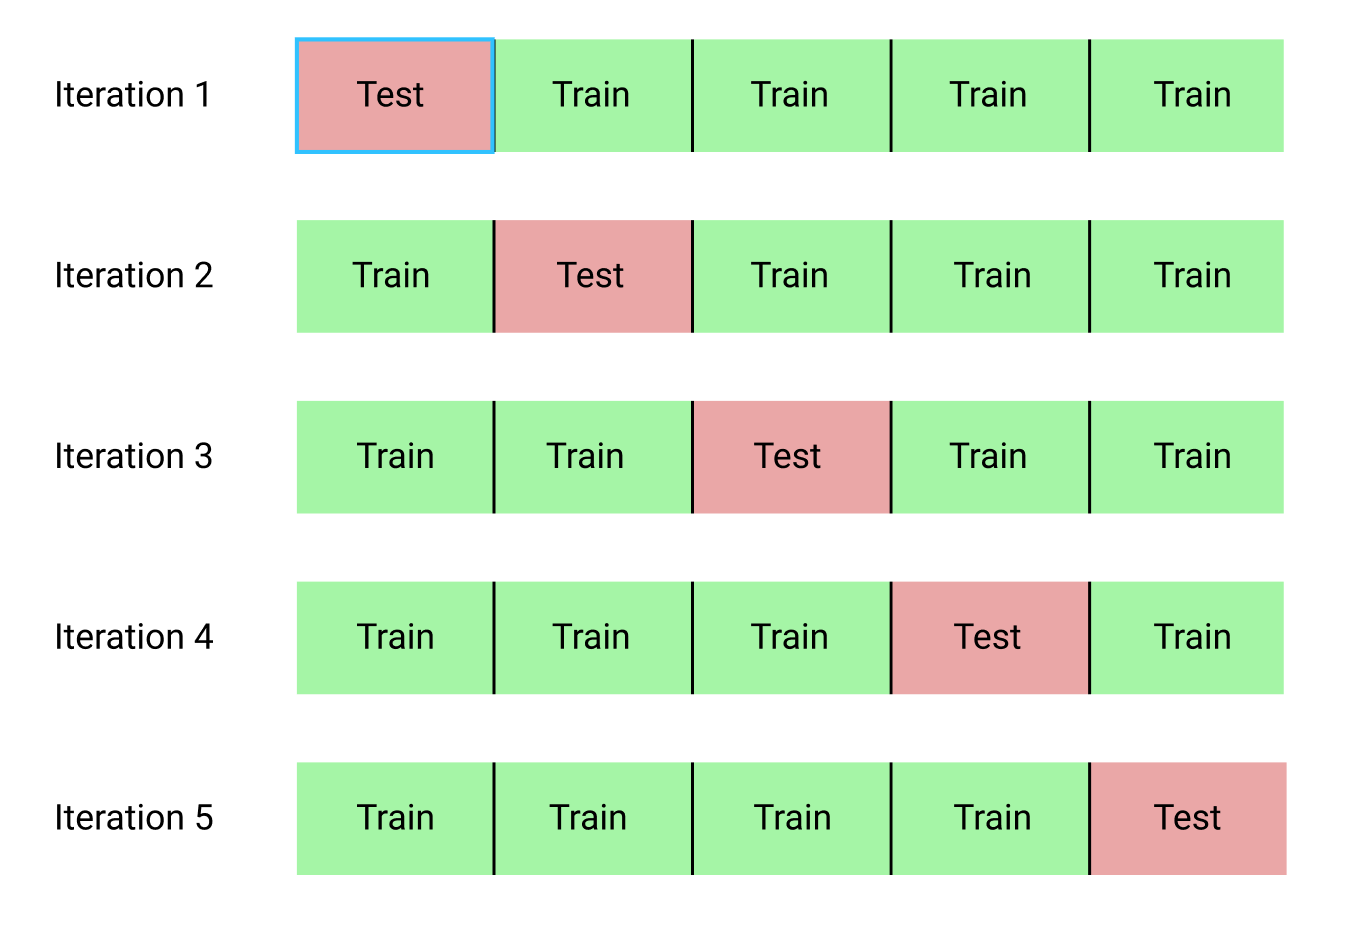
\includegraphics[width=7cm]{img/k-fold1.png}
    \centering
    \caption{Validação cruzada \textit{k-fold}}
    \label{fig:kfold}
\end{figure}

\subsection{\textit{Holdout}}

\textit{Holdout} é um método de atribui de forma aleatórias os dados dentro de dois grupos, conjunto de treinamento e conjunto de teste. Os elementos são escolhidos de forma aleatória para cada grupo, como uma forma de evitar viés na seleção dos dados.  O tamanho dos conjuntos é arbitrário mas via de regra é utilizado um conjunto menor para teste. Uma proporção típicamente utilizada é 80/20, onde 80\% dos dados vão para treinamento e 20\% dos dados vão para teste. Uma comparação do \textit{holdout} com o \textit{k-fold} é mostrado na Figura \ref{fig:holdout1}.

\begin{figure}[h!]
    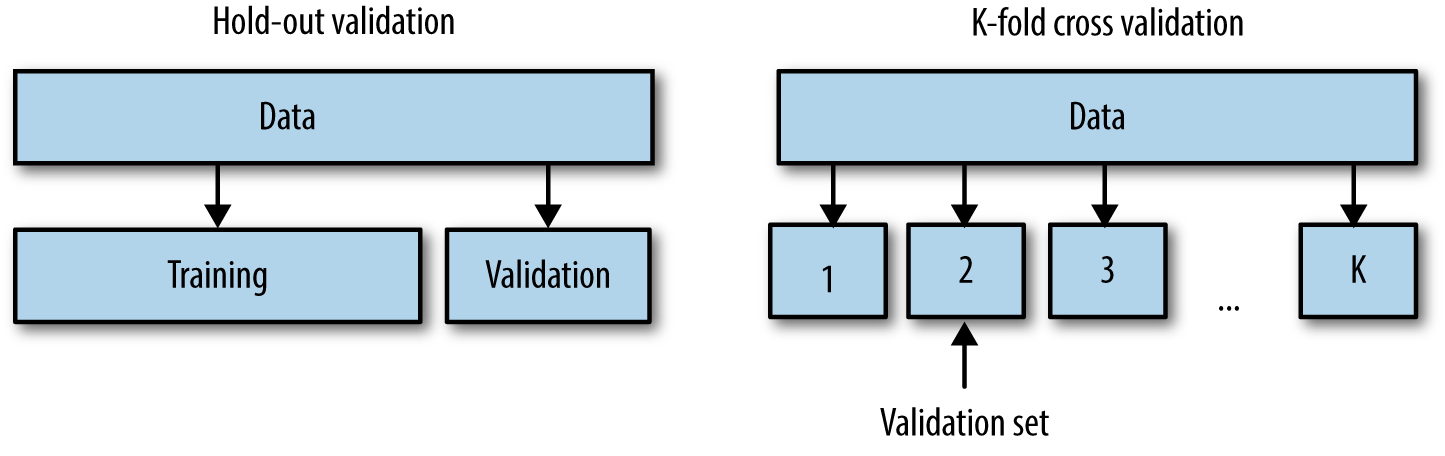
\includegraphics[width=8cm]{img/holdout1.png}
    \centering
    \caption{Validação cruzada \textit{holdout} vs \textit{K-fold}}
    \label{fig:holdout1}
\end{figure}

\section{Classificação}

Em aprendizado de maquina \textbf{classificação} é o problema de categorizar uma amostra nova de acordo com um grupo de categorias. Nessa atividade iremos mostrar diferentes técnicas de classificação nas sub-sessões abaixo.

\subsection{\textit{k-nearest neighbors (KNN)}}

O KNN é um dos primeiros métodos dentro do contexto de classificação devido a sua simplicidade. Em sua versão mais simples, onde K = 1, ele consiste de categorizar o novo dado de acordo com a classe do elemento de menor distância euclidiana dentro do conjunto de treinamento. Para valores maiores de K, são utilizados os K vizinhos mais próximos para definir qual a categoria do dado mais novo.

\subsection{Algoritmo do Centroide mais Próximo}

Similar ao método 1-NN, o algoritmo do centroide mais próximo usa essa mesma estratégia porém essa distancia é calculada de acordo com os contróides dos dados do conjunto de treinamento. O centróide é calculado a partir da média das localizações dos pontos de uma mesma classe. Esse processo é repetido para todas as classes até que exista apenas um ponto para representar cada uma das classes.

\subsection{\textit{Linear discriminant analysis} (LDA)}

LDA é um método de classificação que busca encontrar uma combinação linear das características dos elementos de treino de forma a separar duas ou mais classes. O resultado da separação é uma linha, plano ou hiperplano que divide o conjunto de dados de acordo com a quantidade de características contidas no dado.

Há também a versão \textit{naive} do classificador LDA também conhecida como \textit{naive beyes}. Aqui é assumido que há independencia entre as \textit{features} do banco de dados. O que na prática é usualmente uma suposição incorreta, gerando um pior desempenho na classificação.

\subsection{\textit{Quadratic discriminant analysis (QDA)} (QDA)}

QDA é utilizado em classificação para separar amostras em duas ou mais classes a partir de uma superfície quadrática. A separação das classes é feita por uma parábola, hipérbole, ou planos e hiperplanos que são compostos a partir da junção de outras curvas quadráticas, sendo ele uma versão mais geral do LDA.

O QDA também possui uma versão \textit{naive} como foi explicado na sub-sessão anterior.

\begin{figure}[h]
    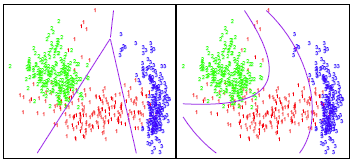
\includegraphics[width=8cm]{img/LDAQDA.png}
    \centering
    \caption{Diferentes curvas de decisão geradas em LDA e QDA}
    \label{fig:ldaqda}
\end{figure}

\newpage

\section{Código e resultados}

Nessa sessão será apresentada informações sobre como foram feitos os algoritmos e também os resultados desses algoritmos aplicados na base de dados \textit{iris\_log}.

\subsection{Programação}

A linguagem de programação utilizada para resolver o problema foi \textit{Python 3.7}. Foram utilizadas as bibliotecas \textit{sklearn} e \textit{numpy} para auxiliar na aplicação das técnicas discutidas na Sessão 1 e também no tratamento de dados, respectivamente. 

A base de dados “iris\_log.dat” contém 150 amostras divididas em 3 classes de 50 amostras cada. Cada amostra da base contém 4 características dada por um valor real.

\subsubsection{1-NN}
O primeiro método utilizado para a classificação dos dados foi 1-NN que obteve os seguintes resultados:

\begin{table}[h!]
\begin{tabular}{l|l|l|l|}
\cline{2-4}
                                                       & Holdout  & K-fold   & Leve-one-out \\ \hline
\multicolumn{1}{|l|}{1-Nearest Neighboor}              & 95.78 \% & 96.00 \% & 96.00 \%     \\ \hline
\multicolumn{1}{|l|}{1-Nearest Neighboor (z-score)}    & 94.00 \% & 95.33 \% & 94.67 \%     \\ \hline
\end{tabular}
\caption{Tabela com diferentes validações cruzadas utilizando 1-NN como classificador}
\end{table}

Vemos que a validação cruzada é bem próxima para diferentes técnicas de divisão de dados, além de ser um bom resultado mostrando que para essa base de dados é possível gerar uma boa classificação utilizando 1-NN.
A normalização dos dados causou uma perda no desempenho do algoritmo.

\subsubsection{Centróide mais próximo}
A utilização de centróide mais próximo na base \textit{iris\_log} gerou os seguintes resultados:

\begin{table}[h!]
\begin{tabular}{l|l|l|l|}
\cline{2-4}
                                                       & Holdout  & K-fold   & Leve-one-out \\ \hline
\multicolumn{1}{|l|}{Centróide mais próximo}           & 93.44 \% & 92.67 \% & 92.67 \%     \\ \hline
\multicolumn{1}{|l|}{Centróide mais próximo (z-score)} & 85.56 \% & 86.00 \% & 84.67 \%     \\ \hline
\end{tabular}
\caption{Tabela com diferentes validações cruzadas utilizando centróide mais próximo como classificador}
\end{table}

O desempenho inferior ao 1-NN é esperado, visto que o centróide mais próximo é uma técnica que reduz a singularidade dos dados a partir do cálculo da média das características dos elementos de uma mesma classe. Novamente as diferentes formas de validação cruzada mostraram resultados próximos, indicando assim que uma estabilidade no método de classificação.
Assim como no 1-NN a normalização dos dados causou uma perda, porém ela foi ainda maior no desempenho do algoritmo de centróide mais próximo.

\subsubsection{ \textit{Linear discriminant analysis} }

Os dados abaixo são resultados da utilização de LDA como método de classificação na base \textit{iris\_log} utilizando diferentes métodos de validação cruzada: 

\begin{table}[h!]
\begin{tabular}{l|l|l|l|}
\cline{2-4}
                                                       & Holdout  & K-fold   & Leve-one-out \\ \hline
\multicolumn{1}{|l|}{LDA}                              & 84.67 \% & 86.00 \% & 85.33 \%     \\ \hline
\multicolumn{1}{|l|}{LDA (z-score)}                    & 85.22 \% & 86.00 \% & 85.33 \%     \\ \hline
\multicolumn{1}{|l|}{LDA naive}                        & 86.22 \% & 86.00 \% & 84.67 \%     \\ \hline
\multicolumn{1}{|l|}{LDA naive (z-score)}              & 85.11 \% & 86.00 \% & 84.67 \%     \\ \hline
\end{tabular}
\caption{Tabela com diferentes validações cruzadas utilizando LDA como classificador}
\end{table}

Os resultados de LDA como classificador se mostrou inferior aos dois métodos previamente vistos, apesar de serem métodos menos complexos. A qualidade dos resultados é diretamente ligada aos dados que estão sendo tratados, nesse caso o LDA não é um algoritmo adequado para essa base de dados, já que ele apresentou o pior resultado em relação aos métodos aqui analisados.

Com exceção do \textit{holdout} onde há uma pequena variância na porcentagem de acerto dependendo do experimento, a normalização dos dados não pareceu influenciar os resultados para esse método de classificação.

Os métodos de LDA \textit{naive} causaram um leve aumento em relação ao LDA tradicional utilizando a validação cruzada \textit{Holdout}, porém uma diminuição em relação ao método de \textit{Leave-one-out}. Entretanto, mesmo utilizando a versão \textit{naive} os resultados continuaram entre os piores do experimento.

\subsubsection{ \textit{Quadratic discriminant analysis} }

Os dados abaixo são resultados da utilização de QDA como método de classificação na base \textit{iris\_log} utilizando diferentes métodos de validação cruzada:

\begin{table}[h!]
\begin{tabular}{l|l|l|l|}
\cline{2-4}
                                                       & Holdout  & K-fold   & Leve-one-out \\ \hline
\multicolumn{1}{|l|}{QDA}                              & 96.89 \% & 96.67 \% & 96.67 \%     \\ \hline
\multicolumn{1}{|l|}{QDA (z-score)}                    & 97.11 \% & 96.67 \% & 96.67 \%     \\ \hline
\multicolumn{1}{|l|}{QDA naive}                        & 95.56 \% & 95.33 \% & 95.33 \%     \\ \hline
\multicolumn{1}{|l|}{QDA naive (z-score)}              & 95.78 \% & 95.33 \% & 95.33 \%     \\ \hline
\end{tabular}
\caption{Tabela com diferentes validações cruzadas utilizando QDA como classificador}
\end{table}

A utilização do QDA gerou um aumento significativo em relação as técnicas de centróide mais próximo e LDA. Seus resultados, dentro dessa base de dados, são os melhores registrados nos experimentos ficando marginalmente acima do 1-NN. 

Assim como no LDA a normalização dos dados não apresentou diferença ao classificar os dados.

A utlização dos métodos \textit{naive} mostraram pior resultado na classificação dos dados.

\section{Conclusão}

Nesse relatório foram utilizados diferentes métodos de classificação, que foram testados utilizando 3 métodos de validação cruzada. As técnicas de classificação podem ser entendidas como 2 tipos, uma de distancia euclidiana entre vetores (1-NN e centróide mais próximo) e a outra que cria uma linha de separação entre os dados (LDA e QDA). Podemos observar que mesmo conceptualmente diferentes ambas apresentaram resultados com mais de 80\% de acerto, com a melhor classificação conseguindo até próximo de 97\% de acerto de acordo com a validação cruzada.
Existe um compromisso entre as diferentes técnicas, onde para bancos de dados muito grandes pode haver um custo computacional muito caro para gerar a classificação, apesar do bom resultado dado pela validação cruzada.

A normalização dos dados se mostrou ineficiente para a base \textit{iris\_log} tendo um pior resultado em todos os diferentes classificadores.

Todo o código desenvolvido para esse trabalho pode ser encontrado em \url{https://github.com/faellacurcio/rp} .

%%% End document
\end{document}